\chapter{Sviluppo Controllo reale}\label{cap:controlDevelop}

\begin{minipage}{12cm}\textit{
		In questo capitolo vedremo come implementare nella realtà il controllore che abbiamo teorizzato all'interno del \microControllore, tareremo i suoi coefficienti e mostreremo come si comporta in un esperimento reale con tutti i problemi ad esso connessi (\nonLinearita del \cite*{IBT-2}, errori di quantizzazione, discretizzazione del controllo, ecc...)
	}
\end{minipage}

\vspace*{1cm}

\begin{figure}[H]
	\centering
	\caption[Impianto Reale]{Impianto Reale}
	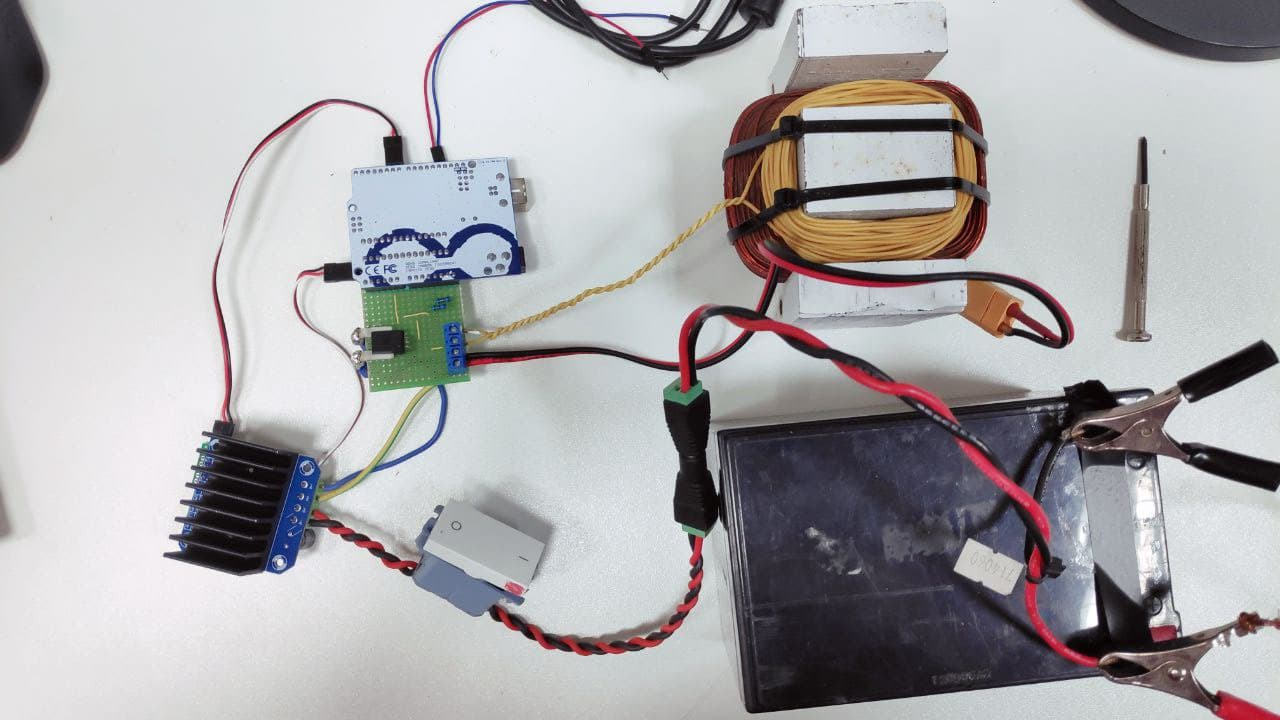
\includegraphics[width=1\textwidth]{ImpiantoReale.jpg}
\end{figure}

\newpage
\noindent
Essendo un \microControllore un computer non eccessivamente potente, è necessario realizzare la funzione di trasferimento del il controllo (equazione \ref{eq:controllerDesign}) mediante un sistema a tempo discreto.\\
Per semplificarci l'implementazione, invece di creare un unico sistema del 2° ordine, si è optato per sommare tra loro le tre funzioni di trasferimento base che lo compongono.\\
Questa scelta è stata presa al fine di semplificare il debugging e permettere un più semplice controllo sullo stato dei sistemi dinamici, possibilità utile nell'ottica di voler saturare gli stati dei singoli integratori una volta che l'uscita ha superato la soglia di attuabilità (\textit{Saturazione}).\\
In fine, essendo l'obiettivo di controllo realizzato da una rampa, dopo un certo tempo in saturazione, per evitare lo spreco di energia da parte della batteria che alimenta il sistema, il codice ha implementato al suo interno un \textit{Safe-Shutdown} che spegne il Ponte-H e resetta tutti gli stati del controllore, oltre che riportare il riferimento da inseguire a 0.\\
Questo stato non è permanente ma persiste fino all'arrivo di un nuovo riferimento da parte del companion esterno, qui simulato dal programma linux \textit{MARTe2Moc}, che comunica con il \microControllore attraverso \cite*{EMP}.

\newpage
\section{Discretizzazione Zero-Order Hold (Z.O.H.)}
Un oggetto del tipo \textit{\textbf{Zero-Order Hold} (Z.O.H.)} altro non è che un convertitore Digitale$ \rightarrow $Analogico che permette di interfacciare dei segnali \textbf{Tempo Discreto} $\mathbb{T} =  \mathbb{Z} $ che evolvono $\forall \Delta T_s $\footnote{$ T_s $ = Sampling Time} con sistemi dinamici \textbf{Tempo Continuo} $\mathbb{T} =  \mathbb{R} $.\vspace{-2mm}
\begin{figure}[H]
	\centering
	\caption[Discretizzazione Zero-Order Hold  $ H_d(z) $ del sistema Tempo continuo $ H(s) $]{Discretizzazione ZOH $ H_d(z) $ per il sistema Tempo continuo $ H(s) $}\vspace{4mm}
	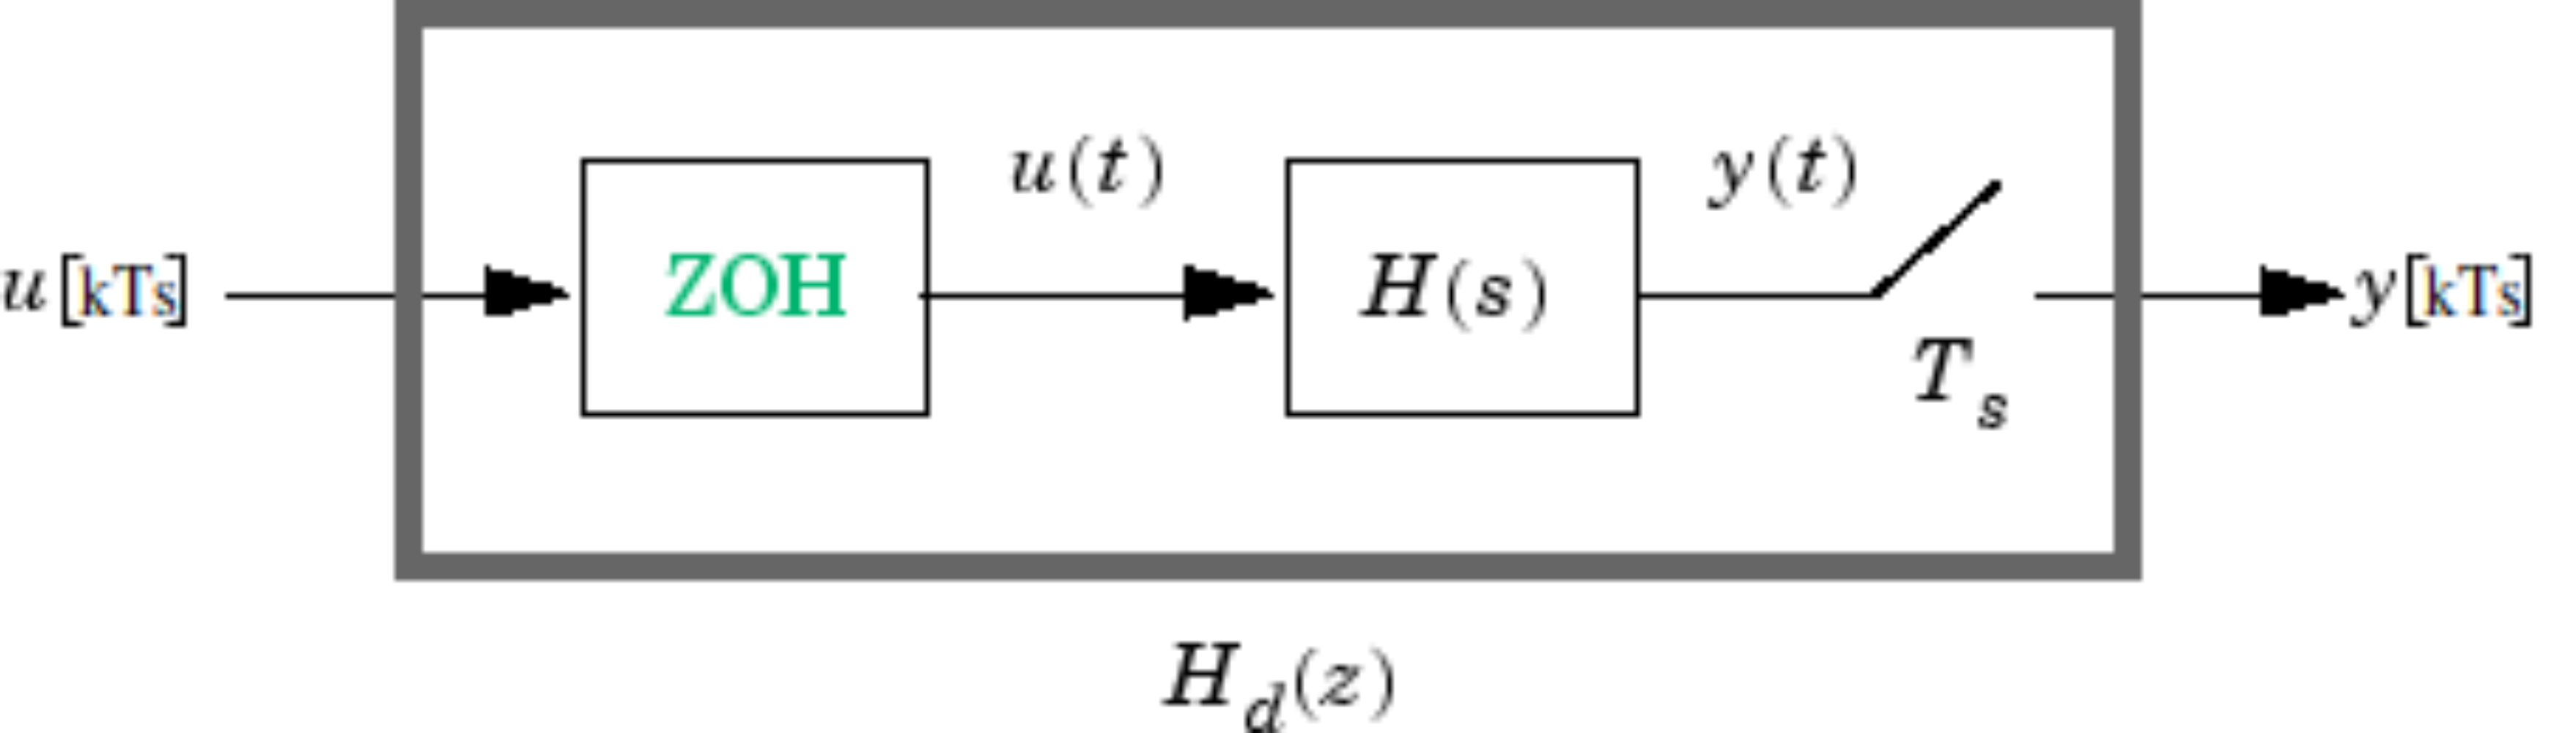
\includegraphics[width=1\textwidth]{Controllo/zoh-apply-Big.png}
\end{figure}\vspace{-6mm}
\noindent
Questa interconnessione "\textit{congela}" l'ultimo segnale discreto $ u(k T_s) $ ricevuto e lo ripropone come un segnale costante in ingresso al sistema continuo che evolve in maniera indipendente.\\
L'uscita $ y(k T_s) $ è la discretizzazione di $ y(t) $, campionata ogni $ T_s $ .
\begin{figure}[H]\vspace{-3mm}
	\centering
	\caption[Effetto sui segnali discretizzati con il metodo Zero-Order Hold]{Segnali discretizzati con il metodo Zero-Order Hold}\vspace{2mm}
	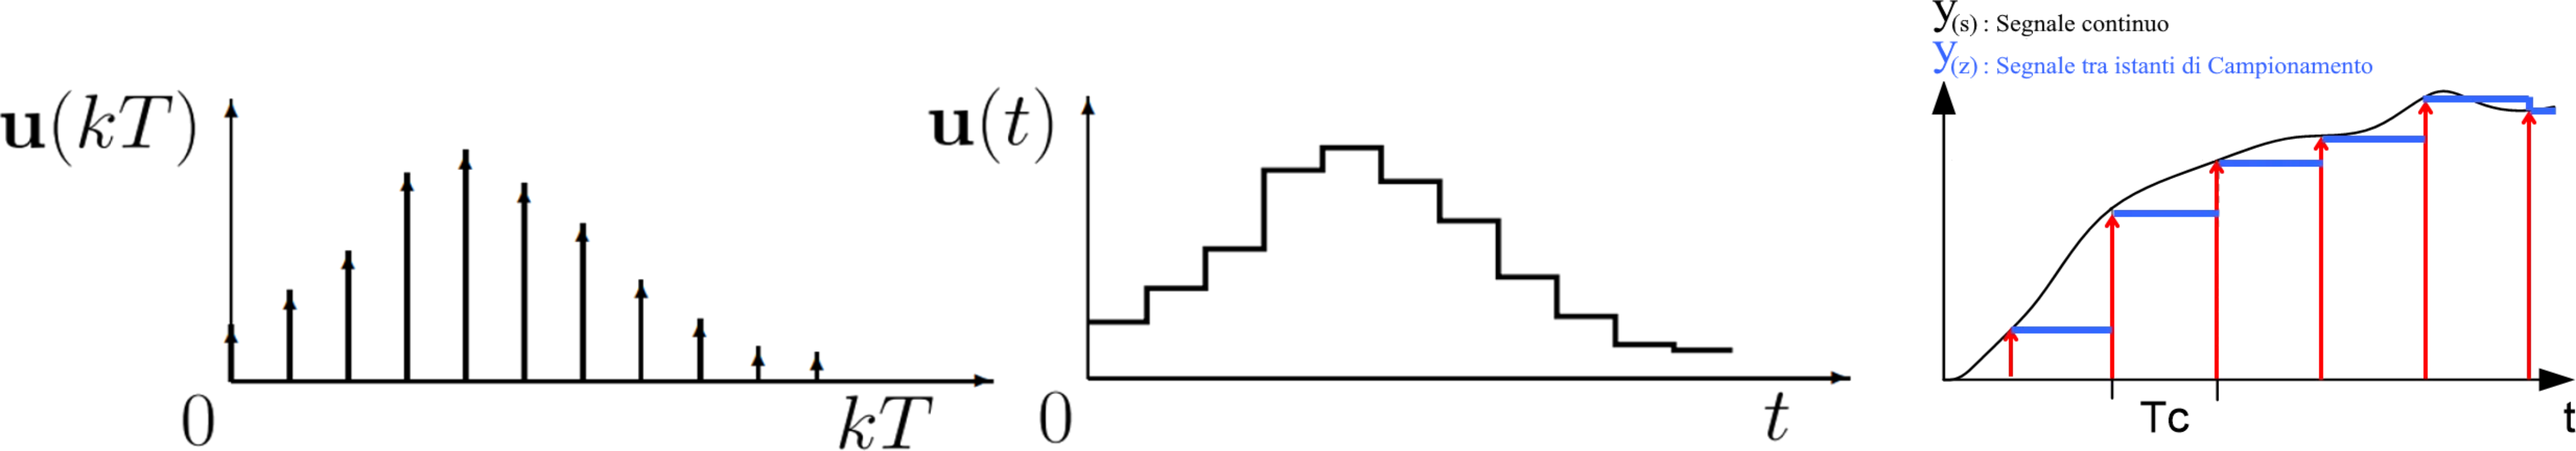
\includegraphics[width=1\textwidth]{Controllo/SegnaliDiscretiContinui-v2-Big.png}
\end{figure}
\noindent
Il sistema $ H(s) $ durante gli intervalli $ T_s $  evolve avendo una costante in ingresso, e al successivo istante di campionamento l'uscita raggiunta viene campionata e mantenuta per ul successivo $ T_s $, e questo procedimento all'infinito.
\newpage
\noindent
Ora che abbiamo descritto qualitativamente cosa avviene usando una discretizzazione ZOH, vediamo ora come diventa $ H_d(s) $ nello spazio di stato in termini matematici. Il procedimento di discretizzazione necessita di passare attraverso lo spazio di stato dei 3 sistemi dinamici che compongono il controllore \ref{eq:controllerDesign} e usando le formule del professore \cite{Discretizzazione}, si ottengono i risultati seguenti risultati:
\begin{table}[H]
	\centering
	\caption[Funzioni di trasferimento nello spazio di Stato, da Tempo Continuo a Tempo Discreto]{Funzioni di trasferimento nello spazio di Stato, da $ \mathbb{T} = \mathbb{R} \rightarrow \mathbb{T} = \mathbb{Z} $}\label{tab:discretizzazione}
	{\Large
		\begin{tabular}[t]{||c||c||c||}
			\hline
			                                                                          &                                        &                         \\[-3mm]
			$ C_{I^2}(s) = \frac{K_2}{s^2}$                                           & $ C_I(s) = \frac{K_1}{s}$              & $ C_p(s) = K_p $        \\[2mm]
			                                                                          &                                        &                         \\[-3mm]
			{\normalsize $ \left\{\begin{matrix}
					\dot{x} = & \begin{pmatrix}
						0 & 1 \\
						0 & 0
					\end{pmatrix} x & + & \begin{pmatrix}
						0 \\
						K_2
					\end{pmatrix} u \\
					          &                                                               \\[-1mm]
					y       = & \begin{pmatrix}
						1 & 0
					\end{pmatrix} x
				\end{matrix}\right. $
			}                                                                         &
			$ \left\{\begin{matrix}
					\dot{x} = & x & + K_1 \cdot u \\
					y       = & x &
				\end{matrix}\right.$

			                                                                          &
			$\left\{\begin{matrix}
					y = K_p \cdot u
				\end{matrix}\right. $                                                                                                   \\[9mm]
			\hline\hline
			                                                                          &                                        &                         \\[-3mm]
			{\normalsize $ \left\{\begin{matrix}
					x^+ = & {\small \begin{pmatrix}
								1 & T_s \\
								0 & 1
							\end{pmatrix}} \cdot x_k & + & K_2 {\small \begin{pmatrix}
						T_s^2/2 \\
						T_s
					\end{pmatrix}} u_k \\
					      &                                                                                                 \\[-1mm]
					y_k = & \begin{pmatrix}
						1 & 0
					\end{pmatrix} \cdot x_k
				\end{matrix}\right. $
			}                                                                         &
			{\normalsize $ \left\{\begin{matrix}
							x^+ = & x_k & + K_1 T_s \cdot u_k \\
							y_k = & x_k
						\end{matrix}\right.$

			}                                                                         &
			$\left\{\begin{matrix}
					y_k        = K_p \cdot u_k
				\end{matrix}\right. $                                                                                                  \\[9mm]
			                                                                          &                                        &                         \\[-3mm]
			$ C_{I^2}(z)|_{T_s} = K_2 \cdot \frac{T_s}{2} \cdot \frac{z+1}{(z -1)^2}$ & $ C_I(z)|_{T_s} = \frac{K_1 T_s}{z-1}$ & $ C_p(z)|_{T_s} = K_p $ \\[2mm]

			\hline
		\end{tabular}
	}%\Large
\end{table}\vspace{-3mm}
\noindent
Si può notare che in tutti e 3 i sistemi si è scelta una realizzazione della funzione di trasferimento nello Spazio di Stato tempo continuo in \textit{Forma Compagna di Osservabilità} (\cite{FormeCanoniche}).\\
Questa scelta non è stata casuale e ha lo scopo di semplificare in futuro la codifica per un sistema di controllo \textbf{Switching nei Coefficienti}, volto a migliorarne ulteriormente le prestazioni, senza dover scalare lo stato in base al cambio dei coefficienti.\\
Questa comoda proprietà è dovuta alla struttura della matrice $ C $, la quale, per variazioni \textbf{istantanee} dei coefficienti $ K_2,K_1,K_p$, non propaga gli effetti sull'uscita $ y(t) $, l'effetto della variazione arriverà in un secondo momento grazie all'integrazione dello stato, che ovviamente evolverà diversamente da prima a causa delle variazioni dei coefficienti. Per avere un idea qualitativa degli effetti dei coefficienti sul sistema complessivo, rifarsi alla sezione "\nameref{sec:designControlloreConclusioni}".\\
I calcoli della trasformata Zeta, sono presenti solo per completezza e sono stati ottenuti usando la classica formula:\vspace{-5mm}
\begin{center}
	{\Large 		$ G(z) = C_d \left(z I - A_d\right)^{-1} B_d + D_d $}
\end{center}
\noindent
Per i nostri scopi noi siamo interessati alle matrici $ A_d,B_d,C_d,D_d $ della conversione, così da implementare esattamente la discretizzazione di ordine Zero del sistema dinamico.\\
\vspace{-6mm}
\section{Codifica del controllore}\vspace{-4mm}
La codifica del controllore \ref{eq:controllerDesign} avviene attraverso le matrici $ A_d,B_d,C_d,D_d $ riportate in tabella \ref{tab:discretizzazione}, con queste matrici è stato costruito la classe di controllo \verb|iiCTRL| riportata in appendice nel codice del controllore (\nameref{lst:controlClassH} e \nameref{lst:controlClassCpp}).\\
La classe viene chiamata all'interno del \nameref{lst:controlLoop} ogni istante di campionamento, e permette la modifica a richiesta del riferimento da inseguire.\\
All'interno della classe è già codificata una la logica di \textit{Safe-Shutdown}, essa viene attivata quando il controllo ha raggiunto la saturazione per un tempo superiore ai 200ms, risulta infatti rischioso e dispendioso tenere connesso il trasformatore, poiché le correnti che scorrono sono dell'ordine dei 10A, e in ogni caso raggiungere gli obiettivi di controllo necessita di una rampa di corrente sul primario, che non si può ottenere se si è già saturato.\\
Questo contatore viene ripristinato a 0 all'arrivo di un nuovo riferimento da inseguire, causando di fatto il ripristino dell'esperimento.

%\newpage

\section{Esperimenti}
Di seguito vengono riportati diversi spari catturati dal sistema in funzione, nella sua interezza, usando al posto di \MARTe, un programma scritto in C++ per Linux chiamato \textit{MARTe2Moc}, quando il resto del sistema verrà controllato, gli stessi input di comando inviati da questa imitazione saranno ricevuti dal \microControllore e attuati in maniera identica.

\subsection{Inseguimento singolo}
In questo "\textit{sparo}" viene impostato il riferimento a $ V_{2_{ref}}=0.5V $ e il controllo insegue prontamente il riferimento, mantenendo l'errore entro margini molto stretti e con una decrescita esponenziale.\vspace{-2mm}
\begin{figure}[H]
	\centering
	\caption[Esperimento singolo $ V_{2_{ref}}=0.5V $]{Esperimento singolo $ V_{2_{ref}}=0.5V $}
	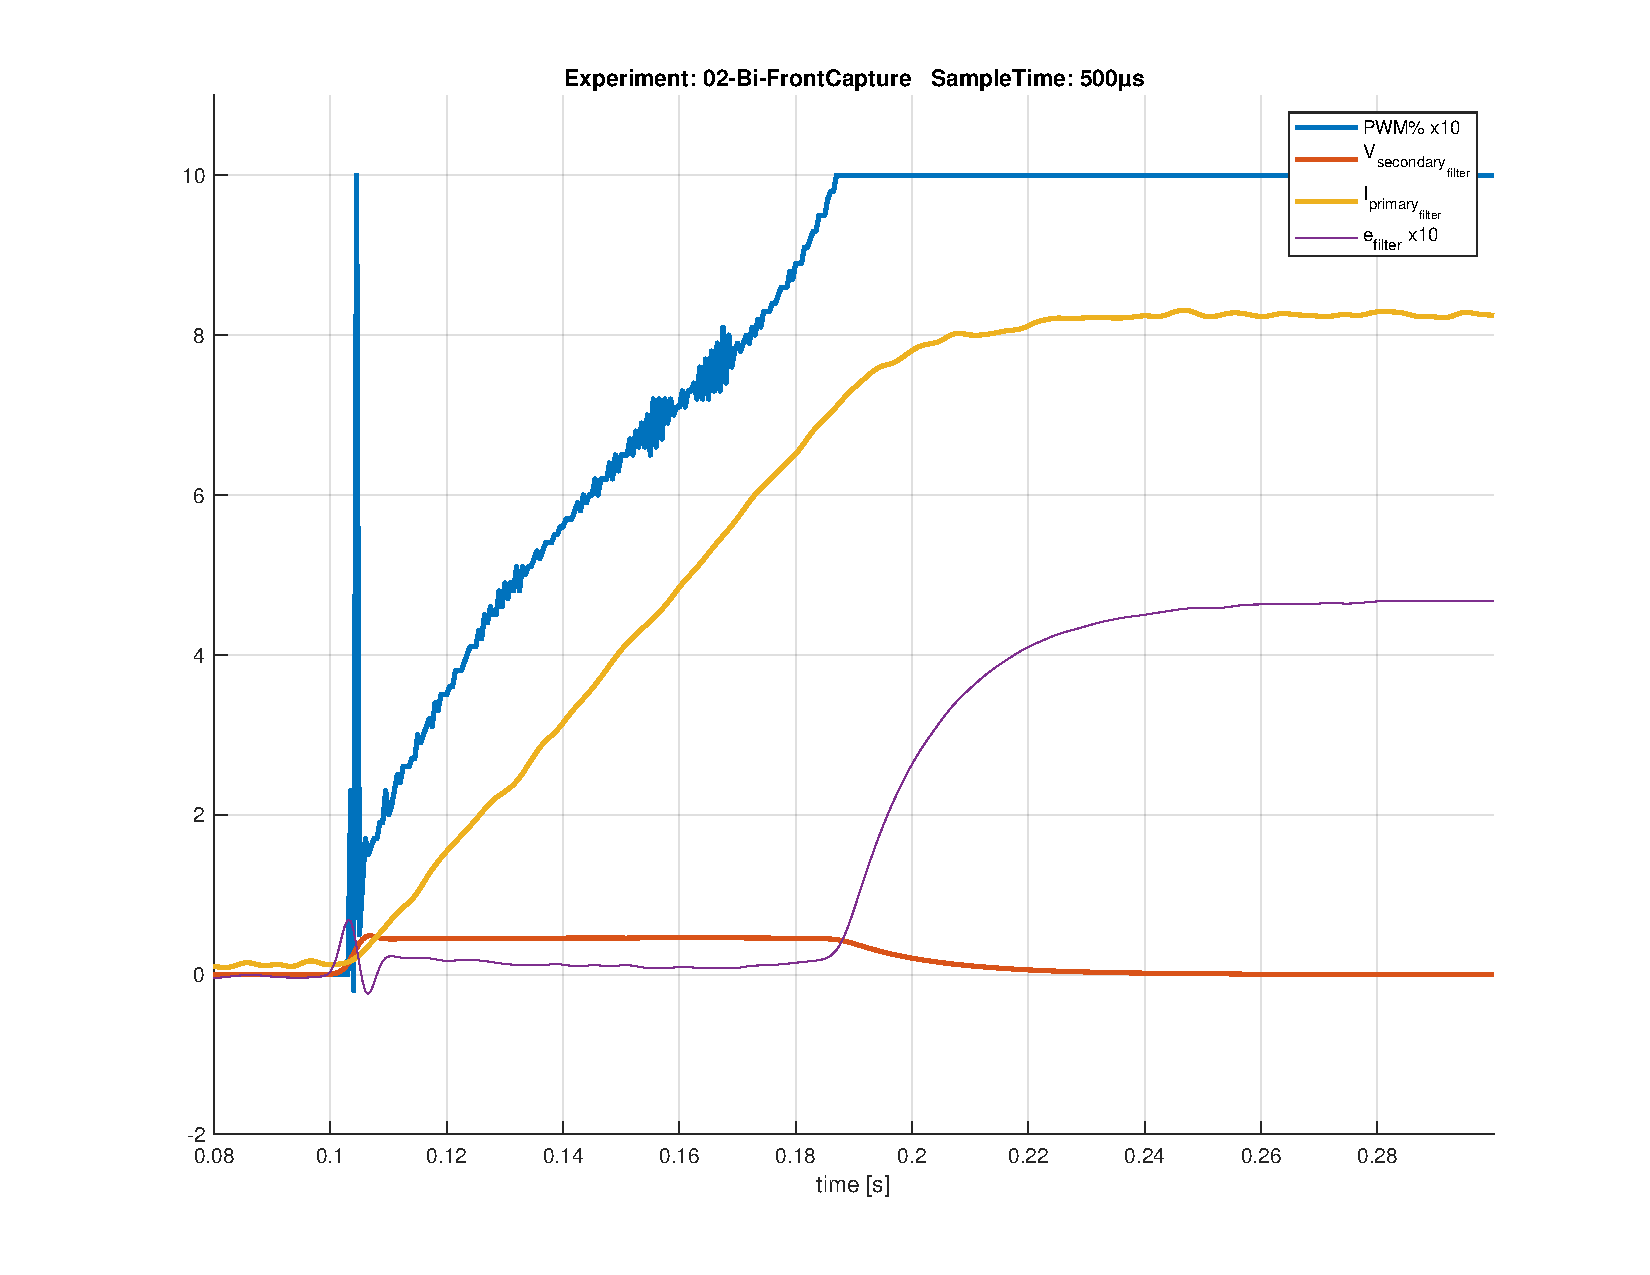
\includegraphics[width=1\textwidth]{Controllo/02-Bi-FrontCapture.pdf}
\end{figure}\vspace{-8mm}
\noindent
Come abbiamo avuto modo di vedere nel capitolo "\nameref{cap:stimaModello}", il modello lineare che abbiamo trovato, taglia tutta una serie di \nonLinearita presenti invece nell'impianto e particolarmente evidenti nei pressi della \textbf{Dead-Zone} e della \textbf{Saturazione}, ma il controllo in catena chiusa riesce a gestire questi problemi e il sistema sin dall'inizio tende a 0 esponenzialmente, la presenza del termine proporzionale permette di reagire immediatamente alla variazione del riferimento, mantenendo l'errore minimo sin dall'inizio.

\subsection{Inseguimento Triangolare}
In questo secondo esperimento, \textit{MARTe2Moc} è stato programmato per invertire il segno del riferimento ogni volta che il controllo arriva in saturazione, l'obiettivo del test è vedere la risposta del controllo nei pressi della \textbf{Dead-Zone} e in corrispondenza di inversione di polarità, il continuo ribaltamento del $ V_{2_{ref}} $ impedisce di arrivare in saturazione troppo a lungo, rendendo l'esperimento periodico e illimitato nel tempo.\vspace{-2mm}
\begin{figure}[H]
	\centering
	\caption[Inseguimento Triangolare $ V_{2_{ref}}=\pm0.5V $]{Inseguimento Triangolare $ V_{2_{ref}}=\pm0.5V $}
	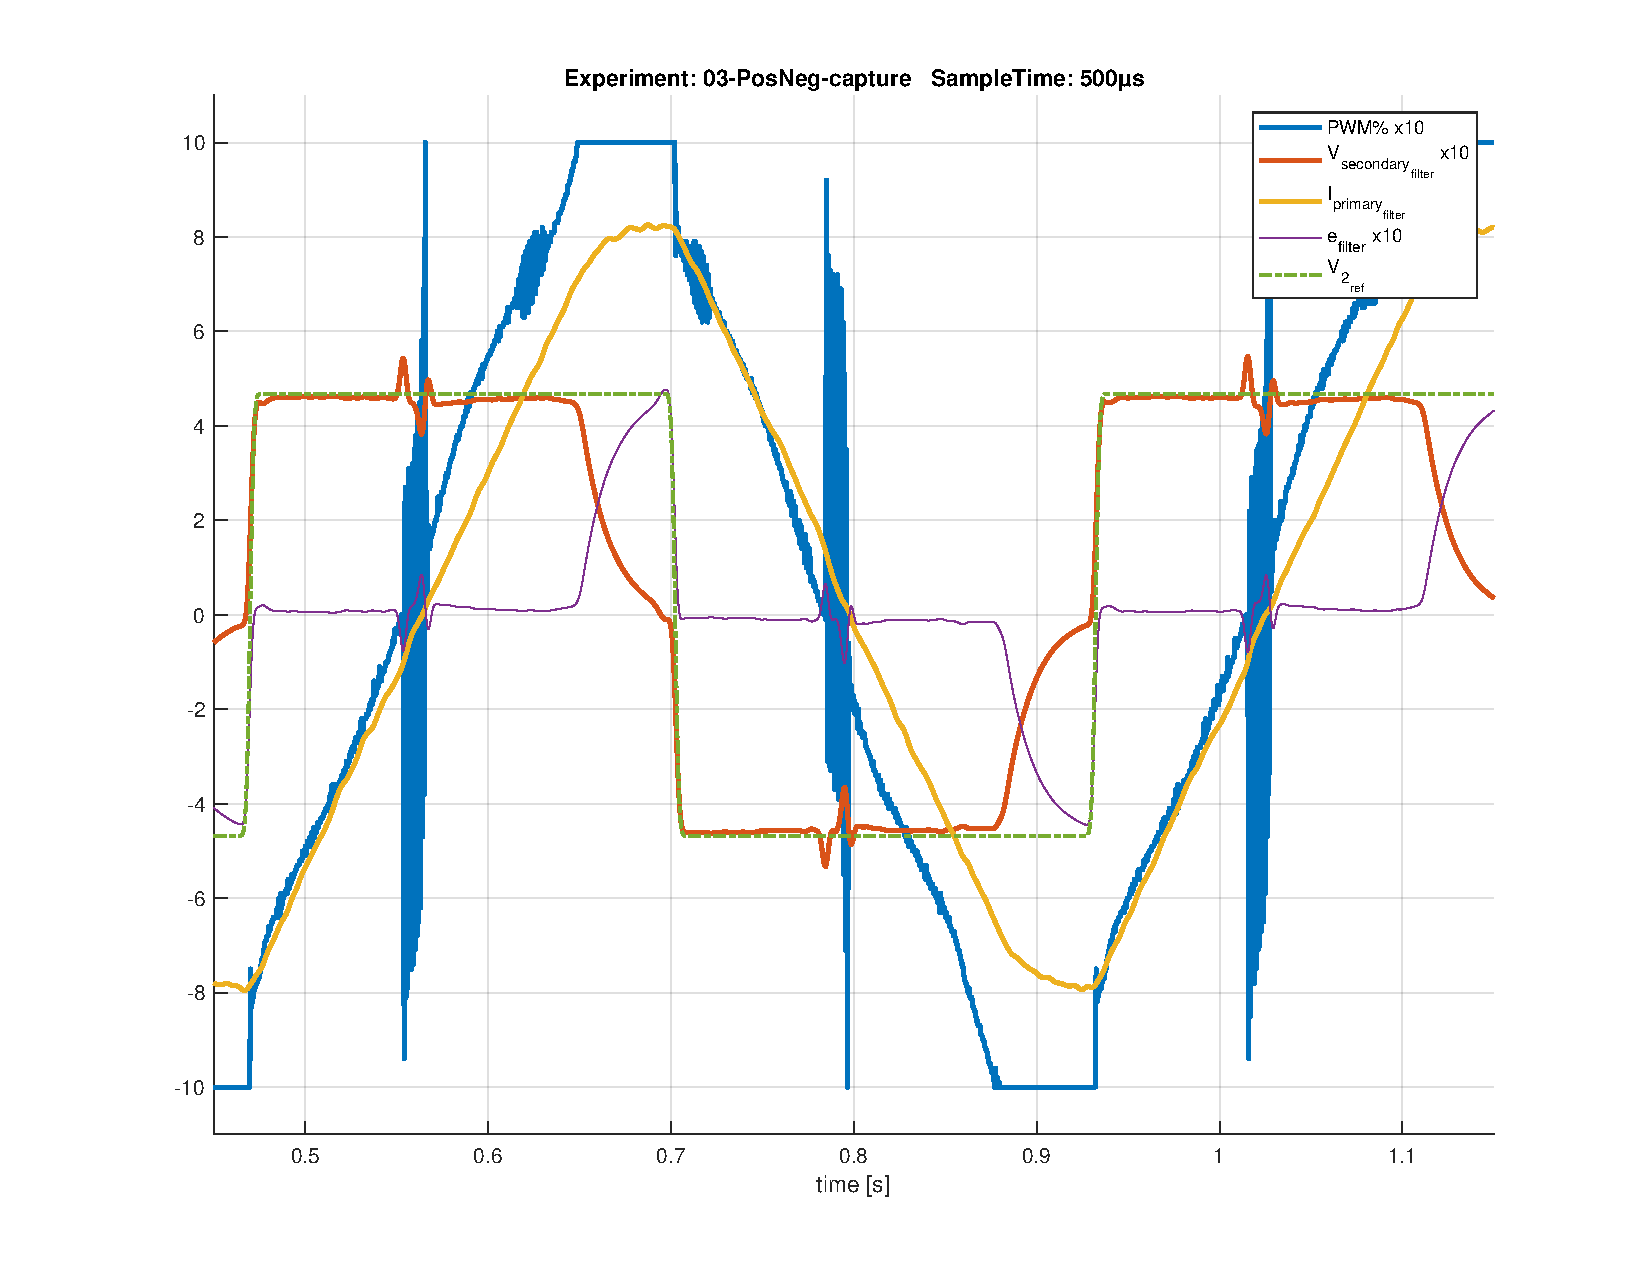
\includegraphics[width=1\textwidth]{Controllo/03-PosNeg-capture.pdf}
\end{figure}\vspace{-8mm}
\noindent
Come è possibile vedere, nei pressi della \textbf{Dead-Zone} la presenza della zona morta fa si che l'errore cresca, ma questa crescita è non superiore a $ 0.02V $, mostrando quanto robusto sia questo design di controllo anche in presenza delle \nonLinearita non modellate nel modello.\\

\newpage

\subsection{Cambio riferimento in corsa}
In questo terzo esperimento, \textit{MARTe2Moc} è stato programmato per inviare un nuovo riferimento casuale, nel grafico riportato vi è stato prima un inseguimento "\textit{lento}", seguito da uno "\textit{ripido}", con una pronta risposta che ha saputo inseguire il cambio mantenendo trascurabile l'errore:\vspace{-2mm}
\begin{figure}[H]
	\centering
	\caption[Cambio di $ V_{2_{ref}} $ prima della saturazione]{Cambio di $ V_{2_{ref}} $ prima della saturazione}
	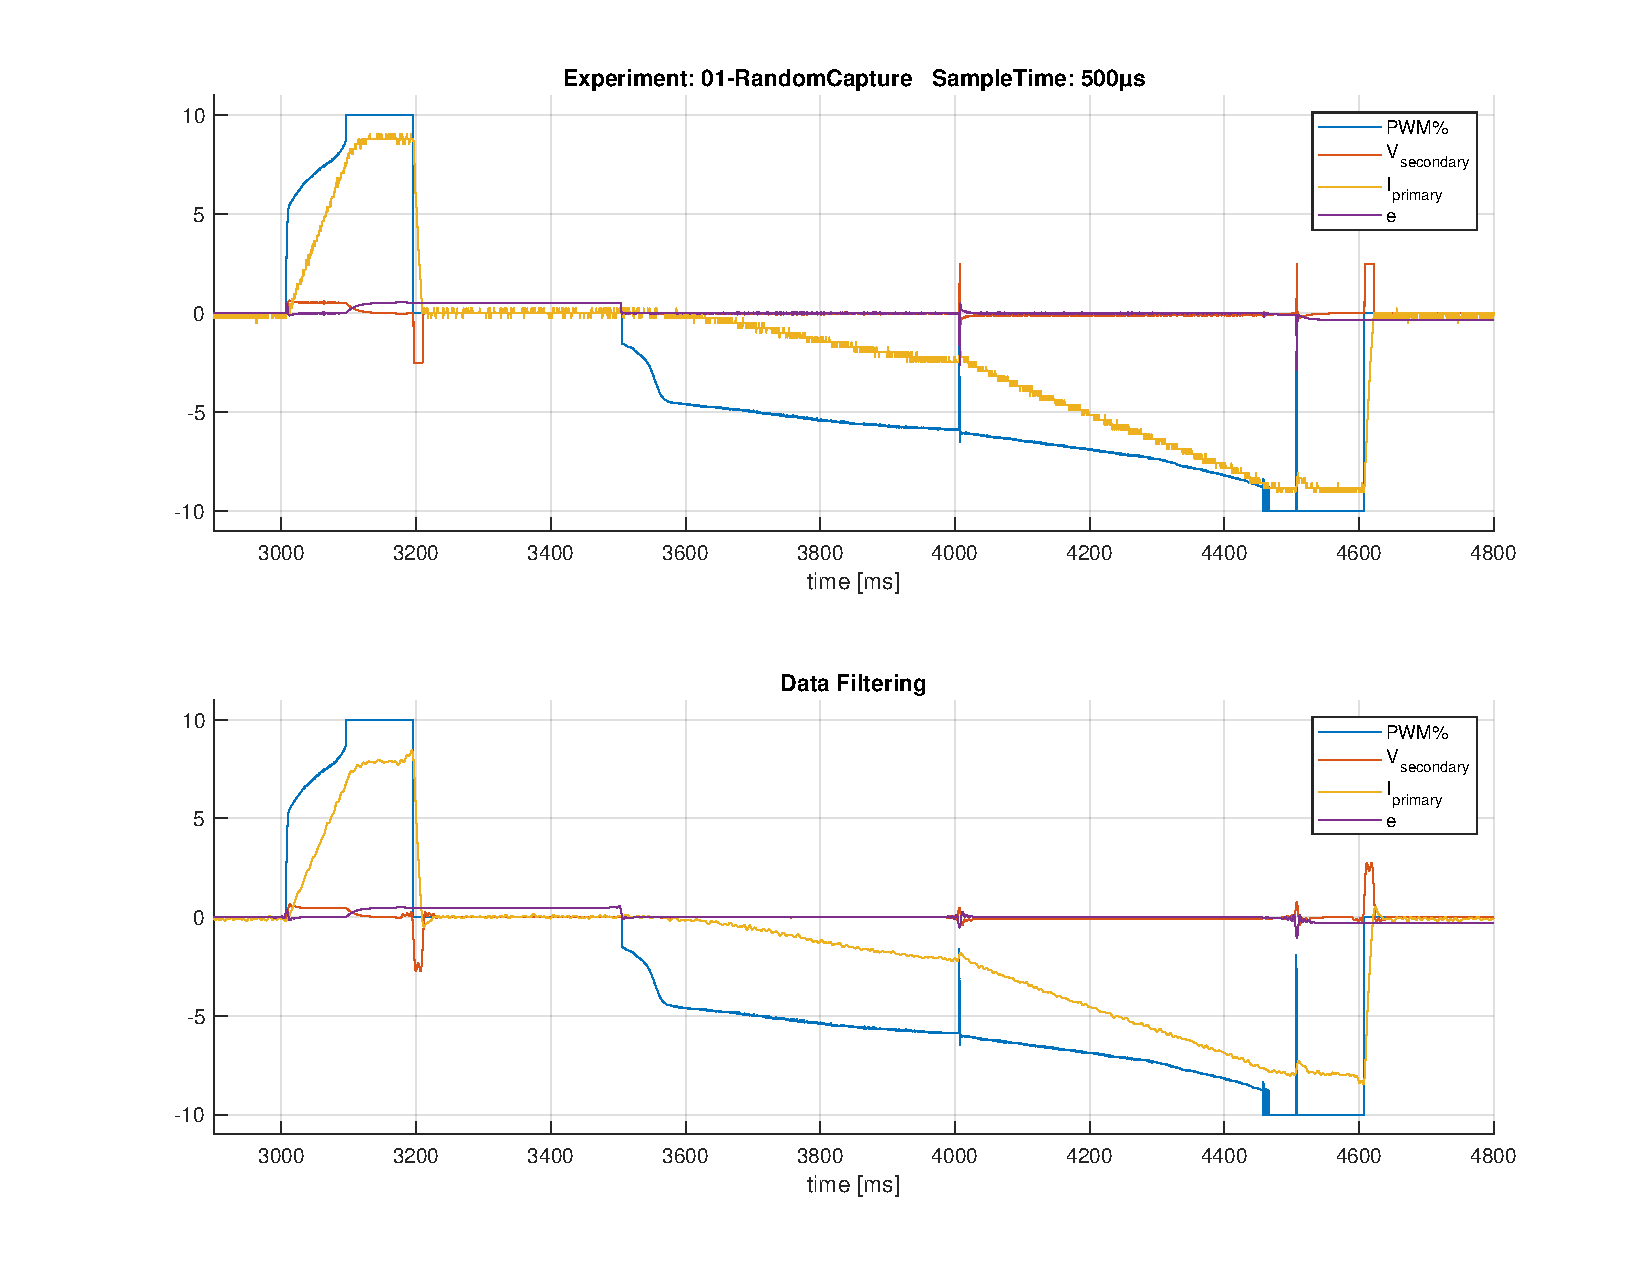
\includegraphics[width=1\textwidth]{Controllo/01-RandomCapture.pdf}
\end{figure}\vspace{-16mm}


\section{Rumorosità nel controllo}
Essendo il controllo in realtà discreto, e soltanto nel range PWM $\in \left[120,200\right] $, è quindi costretto a salire e scendere localmente ad alta frequenza, questo andamento è particolarmente visibile nei pressi delle \nonLinearita da noi trascurate.\\
Il poter avere un controllo in realtà più smooth permetterebbe di migliorare queste oscillazioni e potenzialmente migliorare ulteriormente le performance (già ottime) del sistema aumentando ancora i coefficienti del controllore.